
% !TEX program = xelatex
\documentclass[11pt, a4paper]{report}

% Size of the margins
\usepackage[a4paper,top=3cm,bottom=3cm,left=4cm,right=4cm]{geometry} 
% Font size
% \usepackage[fontsize=1pt]{scrextend}
\usepackage{fontspec}
\setmainfont{Times New Roman}
% For vscode errors
\usepackage{lmodern}
% Language of the text
\usepackage[english]{babel}
% Language for the bibliography
\usepackage[fixlanguage]{babelbib}
% Text encoding
% \usepackage[utf8]{inputenc} 
% Text encoding
% \usepackage[T1]{fontenc}
% Allows you to generate dummy text. It was useful to me
% to understand what the setting of the
% text on the page before I wrote a certain paragraph
\usepackage{lipsum}
% To rotate images
\usepackage{rotating}
% To change the page header
\usepackage{fancyhdr}               

% Mathematical libraries
\usepackage{amssymb}
\usepackage{amsmath}
\usepackage{amsthm}         

% Use of images
\usepackage{graphicx}
% Use of colors
\usepackage[dvipsnames]{xcolor}         
% Using listings for code
\usepackage{listings}          
% To insert hyperlinks between the various elements of the text
\usepackage{hyperref}     
% Different types of underlines
\usepackage[normalem]{ulem}
% remove indent
\setlength\parindent{0pt}


% -----------------------------------------------------------------

% Change the header style
\pagestyle{fancy}
\fancyhf{}
\fancyfoot[C]{\thepage}
\renewcommand{\headrulewidth}{0pt}

% Removes the page number at the beginning of chapters
% \fancypagestyle{plain}{
%   \fancyfoot{}
%   \fancyhead{}
% }

% Code style
\lstdefinestyle{codeStyle}{
    % Comments color
    commentstyle=\color{teal},
    % Color of the keywords
    keywordstyle=\color{Magenta},
    % Line number style
    numberstyle=\tiny\color{gray},
    % Color of the strings
    stringstyle=\color{violet},
    % Text size and style
    basicstyle=\ttfamily\footnotesize,
    % newline only at whitespaces
    breakatwhitespace=false,     
    % newline yes / no
    breaklines=true,                 
    % Position of the caption, top / bottom
    captionpos=b,                    
    % Preserves spaces in code, useful for indentation
    keepspaces=true,
    % Where to display line numbers
    numbers=left,
    % Distance between line numbers
    numbersep=5pt,
    % Show whitespace or not
    showspaces=false,
    % Show whitespace in strings
    showstringspaces=false,
    % Show tabs
    showtabs=false,
    % Size of tabs
    tabsize=2
} \lstset {style = codeStyle}

% Code style for larger size, where I needed smaller text (for example if you want to insert code that has very long lines). To use this style rather than the previous one, use

% \lstset {style=longBlock}
%% enter code ...
% \lstset {style=codeStyle}

% The second command returns to the previous style
\lstdefinestyle{longBlock}{
    commentstyle=\color{teal},
    keywordstyle=\color{Magenta},
    numberstyle=\tiny\color{gray},
    stringstyle=\color{violet},
    basicstyle=\ttfamily\scriptsize,
    breakatwhitespace=false,         
    breaklines=true,                 
    captionpos=b,                    
    keepspaces=true,                 
    numbers=left,                    
    numbersep=5pt,                  
    showspaces=false,                
    showstringspaces=false,
    showtabs=false,                  
    tabsize=2
} \lstset{style=codeStyle}

% By removing the comment on the following command, the sources present in Bibliography.bib but not directly cited with the \ cite command are also inserted in the bibliography
% \ nocite {*}

% Margins before and after blocks of code, to have more distance
\lstset{aboveskip=20pt, belowskip=20pt}

% Change the style of the references, with the text in cyano
\hypersetup{
    colorlinks,
    linkcolor=black,
    citecolor=black
}

% Added definitions, theorems, line and listing
\newtheorem{definition}{Definizione}[section]
\newtheorem{theorem}{Teorema}[section]
\providecommand*\definitionautorefname{Definizione}
\providecommand*\theoremautorefname{Teorema}
\providecommand*{\listingautorefname}{Listing}
\providecommand*\lstnumberautorefname{Linea}

\raggedbottom

%\newcommand{\cgs}[1]{{\textcolor{brown}[\textcolor{red}{\bf{GS: }}{ \textcolor{brown}{#1]}}}}             
%\newcommand{\cmc}[1]{{\textcolor{blue}[\textcolor{magenta}{\bf{MC: }}{ \textcolor{blue}{#1]}}}}



% -----------------------------------------------------------------
\begin{document}

\begin{titlepage}
\begin{figure}[!htb]
    \centering
    
\includegraphics[keepaspectratio=true,scale=2]{images/Frontpage/sustlogo.png}
\end{figure}

\begin{center}
    \LARGE{SHAHJALAL UNIVERSITY OF SCIENCE AND TECHNOLOGY}
    \vspace{5mm}
    \\ \LARGE{Institute of Information and Communication Technology}
    % \vspace{5mm}
    % \\ \LARGE{SWE 420}
\end{center}

\vspace{15mm}
\begin{center}
    {\LARGE{\bf SWE 420\\ \vspace{5mm} Report of Internship }}
    
    % Se il titolo è abbastanza corto da stare su una riga, si può usare
    
    % {\LARGE{\bf Un fantastico titolo per la mia tesi!}}
\end{center}
\vspace{30mm}

\begin{minipage}[t]{0.47\textwidth}
	{\large{Submitted By:}{\normalsize\vspace{3mm}
	\bf\\ \large{Shakirul Hasan Khan} \normalsize\vspace{2mm} \\ 2017831034}}
\end{minipage}
\hfill
\begin{minipage}[t]{0.47\textwidth}\raggedleft
	{\large{Performed At:}{\normalsize\vspace{3mm} \bf\\ \large{Kaz Software}\normalsize\vspace{2mm}\\ 35/5, Shantinagar, Dhaka-1217}}
\end{minipage}

\vspace{30mm}
\hrulefill
\\\centering{Date of Submission: 26 June, 2022}

\end{titlepage}
\chapter*{Letter of Transmittal}

July 16, 2022\\
The Director\\
Institute of Information and Communication Technology\\
Shahjalal University of Science and Technology\\
Sylhet, Bangladesh\\

Dear Sir,

I am very much delighted to submit a report as a part of my internship program.
I am so thankful to the Institute of Information and Communication Technology, SUST for giving me the opportunity to connect my academic knowledge with the latest software development trends in a renowned software industry and to gather great industry experience.

I have been working as an intern at Kaz Software as a part of our course SWE 420, starting from September 1, 2021, to February 28, 2022.
This report is based on my learning and experience during my internship time period. And this report covers the technical skills I developed during my internship program as well as my project participation, skill acquisition, and other improvements and issues.

I believe this report will be able to summarize the overall outcome of my internship course.
I will be grateful if you accept my report, and your consideration will be highly appreciated.\\

Sincerely yours,
\begin{figure}[h]
    
\includegraphics[width= 0.25\textwidth]{images/LetterOfTransmittal/mySignCropped.jpg}  
    \label{fig:mySign}
\end{figure}
\hrule height 0.4pt width 120pt
\vspace*{15pt}
Md. Shakirul Hasan Khan Mobin\\
Registration No: 2017831034\\
Department of Software Engineering\\
Institute of Information and Communication Technology\\
Shahjalal University of Science and Technology
\chapter*{Letter of Endorsement\\{\Large\normalfont To whom it may concern}}

% (To whom it may concern)\\\\
\textbf{Subject:} Approval of the report
\vspace{40pt}

This is to certify that all the information mentioned in the report is accurate and not confidential to the company.
Shakirul Hasan Khan had direct involvement in the projects mentioned in the report.

I personally went through and examined every page of the report, and I was unable to locate any information that contravened the organization's privacy policies.

I therefore declare the report to be true and give Shakirul Hasan Khan my best wishes for a prosperous future.

\vspace{75pt}
\setlength{\tabcolsep}{15pt}
\begin{center}
    \begin{tabular}{ccc}
    \cline{1-1} \cline{3-3}
    \begin{tabular}[c]{@{}c@{}}\\Shawal Siddique Shaon\\Chief Technology Officer\\Kaz Software\end{tabular} & & \begin{tabular}[c]{@{}c@{}}\\Md. Hannan Hossain\\Principal Software Engineer\\ Kaz Software\end{tabular}
    \end{tabular}
\end{center}

\chapter*{Acknowledgement}

I am excited to share this report about my internship experience at Kaz Software.
I want to express my sincere gratitude to the Institute of Information and Communication Technology, SUST, for providing an opportunity for my internship.
I also want to express my regards to Kaz Software for the support and the opportunity to work with a great team.\\

I would like to thank Shawal Siddique Shaon, CTO of Kaz Software, for his guidance and support throughout the internship period.
I would also like to thank my mentors, Md. Hannan Hossain (Principal Software Engineer) and Biswajit Panday (Senior Software Engineer), who trained and guided me in my internship journey.\\

I would also like to thank Ibrahim Khan Arshad (currently working as a software engineer at Cefalo Bangladesh Ltd.) for his kind assistance and support.
Finally, I want to express my gratitude to my team members, my fellow interns, and every member of Kaz Software for making my internship experience a memorable one.
\chapter*{Executive Summary}

This report serves up the purpose of a summary of the work that I undertook as well as my experience during my internship period which was conducted on Kaz Software.

\tableofcontents

% Remove if you do not want the table of figures
% \listoffigures

\chapter{Introduction}

An internship is a professional learning experience that offers meaningful, practical work related to a student’s field of study or career interest.
An internship gives a student the opportunity for career exploration and development, and to learn new skills.
It offers the employer the opportunity to bring new ideas and energy into the workplace, develop talent and potentially build a pipeline for future full-time employees.
Internships are usually offered part-time if it is during a university semester, or full-time if it is during a vacation.
And in most of the cases, the internship is paid. \\

Institute of Information and Communication Technology, SUST always emphasizes industry knowledge on academic study. 
And to give students actual industry experience, IICT provides the opportunity to their students of Department of Software Engineering to work as an intern for six-months in a renowned software company as a part of their academic curriculum in the 7th semester.
This opportunity helps to add a great value to personal qualification and experiences of their students. \\

The company I was sent to for my internship is Kaz Software. It is one of the most experienced software company in Bangladesh. Kaz Software have been successfully operating for more than 18 years.

\section{Objective}

This report is prepared as a requirement of the course SWE 420 at Department of software Engineering, Institute of Information and Communication Technology, SUST. \\

This document is intended to contain achievement, learnings, professional growth, achievements, and overall industrial experience during my internship period. \\

And if it is allowed, this document will be open to other students who'll be working as interns in future.
So that they can decide if Kaz Software is a good choice for them.

\section{Scope}

The main scopes of this document are:

\begin{enumerate}
    \item Work environment and culture of Kaz Software
    \item Experiences I faced as an intern of Kaz Software
    \item Projects I have worked on during my internship
    \item The training and guidance I received
    \item My professional and technical growth
    \item Description of the technologies I used during my internship
    \item And my opinion on this internship
\end{enumerate}

Everything is discussed in this document without violating the confidentiality of the company.

\section{Sources of Information}

All of the information reported in this document is true and authentic.
The accuracy and confidentiality of the information related to the company is verified by executives of Kaz Software.\\

This document contains both technical and theoretical information.
As a result some information is taken from various websites, and the links to that websites are attached at the end of this report.
So that reader can manually verify any external information, if they have any doubt.

\section{Limitations}

There are some limitations in this report.
Not everything I did during my internship period can be shared with outside world.
This document is reviewed by an executive from my company several times before submitting.
And during those reviews, several information have been omitted, because they are confidential to Kaz Software.
As a result this document is not perfect.
\chapter{Company Profile}

This chapter describes the customs and culture of Kaz Software.
Each section describes the overview of Kaz Software, the way it operates, what services they provide, technology used here, key features, location and what people here does for recreation. 

\section{Company Overview}

Kaz Software is one of the best and most experienced software company in Bangladesh.
It started as a start-up software outsourcing company in \textcolor{red}{8 June, 2004} and became a limited company in 2005 and continued to develop year after year.
Typically Kaz Software builds software for the clients, but sometime they would be doing something completely different like researching business data or setting up their firewall.
Kaz Software has some really talented engineers, designers, and content specialists to give it's clients a well built software.

\begin{figure}[h]
    \begin{center}
        
\includegraphics[width=0.9\textwidth]{images/Chapter2/cto_tour.png}
        \label{fig:CTO_Tour}
    \end{center}
\end{figure}

\section{Services}

Kaz Software offers software development and content management services to international customers across multiple industries.
Kaz understands the challenges that its customers face within and across these industries.
Kaz provides practical, pragmatic and powerful solutions to address those challenges.

\begin{figure}[h]
    \begin{center}
        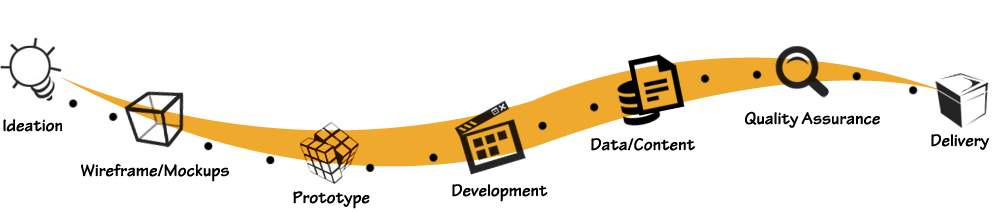
\includegraphics[width= 0.8\textwidth]{images/Chapter2/kaz_services.png}  
        \label{fig:kazServices}
    \end{center}
\end{figure}

The services of Kaz Software covers every step of software development, from ideation to delivery.

\subsection{Ideation, Graphics and Interaction Design}

The design team in Kaz software helps the clients through the digital design and strategy maze.
They work through every stages of a project with the client and keep brainstorming and create mockups, demos and presentations.
And during interaction design, Kaz Software always prefer to create the simplest solution.

\subsection{Software Development}

Teams at Kaz Software help our customers build  customized software - everything from web to desktop to enterprise to mobile and beyond. 
They have been building softwares for various industries since 2004 and worked with many technology platforms and have collaborated with many teams over these years. \\

Kazians have worked on web applications, created desktop applications, and built numerous mobile applications. Some of things that they have built:

\begin{enumerate}
    \item Social app with localization
    \item Desktop based tax optimization tool
    \item Corporate data management application
    \item Document repository
    \item Database driven file system
    \item Content rich web application
    \item LDAP management tool
    \item iPhone/Android/Windows mobile applications
    \item Online holiday management tool
    \item Location content service
    \item Location based social app platform
    \item Flex based visio like diagramming tool
    \item Desktop based diagramming and layouting tool.
    \item Symbian application
    \item VoIP billing solution
    \item Mobile content solution
    \item Stock trading portal
    \item International trade research and management tool
\end{enumerate}

Kazians don't specialize in particular technologies, but they are definitely proficient ein wide array of tools and systems.
Every product is unique, and they try to fit the right skills for that particular product.

\subsection{Quality Assurance}

Integrated quality assurance approach of Kaz Software incorporates aspects of agile and lean development with the stability and reliability of traditional SQA process.
They believe software quality assurance is only possible with a mixed set of procedures which should involve all members of the team collaborating with a dedicated team of SQA professionals.
Because of their involvement with all kinds of projects their SQA teams are exposed to a variety of technology and business domains.
Types of testing services Kaz Software provides:

\begin{enumerate}
    \item Product testing
    \item Performance and Load testing
    \item Content Validation Testing
\end{enumerate}

\subsection{Data, Content and Research}

Kazian research teams have researched, compiled and maintained content in diverse fields and for a variety of applications.
The research team is supported by our data specialists who leverage technology to optimize data gathering and ensure that the data is stored and managed efficiently.
Services provided on this area by Kaz Software:

\subsubsection*{Research}

\begin{enumerate}
    \item Research and compile information
    \item Categorize existing content
    \item Meta tag content
    \item Search and collect publicly available documents
    \item Professional domain based translation of information
    \item Statistical and economic analysis
    \item News gathering and summarizing
\end{enumerate}

\subsubsection*{Create and Maintain}

\begin{enumerate}
    \item Write, edit, proof read content
    \item Maintain content in blogs, CMS or other systems
    \item Translate existing content
    \item Create and maintain structured content like spreadsheets
    \item Maintain newsletters/news services
\end{enumerate}

\subsubsection*{Data Services}

\begin{enumerate}
    \item ransformation of existing data to and from various formats such as csv, xml, etc.
    \item Extracting data from unstructured or structured sources
    \item "Cleaning" data by removing errors, unwanted information etc.
    \item Storage solutions - Databases, XML, flat file
\end{enumerate}

\section{Human Resource}

Kaz has 110+ employees at this moment and they are planning to recruit more.
Since the beginning, Kaz has grown in numbers of resources and production every year.
Kaz doesn't hire developers, designers or QA engineers.
Kaz hires people who solve problems.
And it hires only the best.
Kaz runs regular training and review sessions to keep it on the top.

\section{Facilities for Employees}

Kaz Software always keeps the happiness of their employees at the top priority.
As a result they provide a lot of facilities to keep the Kazians happy.

\subsection{Friendly Environment}

Kaz Software is like one big Family.
Work is fun here.
The work environment here is friendly, informal, fun and knowledge oriented.
Chain of command is not followed here.
Employees consider the company to be their own responsibility.

\subsection{Vacation and Optional WFH}

Kaz Software provides 17 days of paid vacation per year. 
A Kazian can take a full day or half day leave anytime, until it exceeds total of 17 days per year.\\

Another great initiative by Kaz Software is an employee can either go to office or work from home, it's up to them.
And any kind of technical support will be provided no matter where you are, home or office.
Although working from office is more fun because of the friendly environment.

\subsection{Lunch and Snacks}

Kaz Software does not provide any lunch or snacks except tea and coffee.
An employee can go and make their own tea or coffee or ask a Shoinik to make them one.

\subsection{Indoor and Outdoor Games}

Almost every Kazian is a cricket lover.
They play short-pitch cricket every working day after lunch, in the office premises.
There is a table tennis board in the ground floor and Kazians can play anytime they want.

\textcolor{red}{\LARGE Images Goes Here}

\subsection{Recreation}

Kaz has different ways for recreation of employees.
Release parties, picnics, ’Hudai party’, and outings are part of it.
Every year in December Kaz organizes their anniversary party.
Which is either taking all of the employees for an international trip, or a 7 to 10 days trip inside Bangladesh.
And this is fully paid by the office.
In spite of being an intern, I received all these facilities and consider myself lucky.

\subsection{Bonuses and Increment}

Kaz Software does not provide any festival bonus.
But they provide a bonus equal to the salary of a employee after every anniversary of their joining and they get a increment of 10 to 15 percent of their current salary.
This may vary according to an employee's performance.

\appendix

\chapter{References}

\begin{enumerate}
    \item Kaz Software: \url{https://kaz.com.bd/}
    \item Our Services: \url{https://kaz.com.bd/services/}
    \item Our Culture: \url{https://kaz.com.bd/company-culture}
    \item Typescript: \url{https://www.typescriptlang.org/}
    \item ReactJS: \url{https://reactjs.org/}
    \item Redux: \url{https://redux.js.org/}
    \item Git: \url{https://git-scm.com/}
    \item Visual Studio Code: \url{https://code.visualstudio.com/}
    \item Single SPA: \url{https://single-spa.js.org/}
    \item Cypress: \url{https://www.cypress.io/}
    \item Docker: \url{https://www.docker.com/}
    \item Kubernetes: \url{https://kubernetes.io/}
    \item Prothom Shurjo: \url{https://www.facebook.com/ProthomSurjoBD}
    \item Micro-Frontends POC: \url{https://github.com/KhanShaheb34/react-microfrontends/}
\end{enumerate}


% \bibliographystyle{plain}
% \bibliography{chapters/Biblio.bib}

\end{document}
% -----------------------------------------------------------------
